\section{General Astronomy}
Some things we come across that aren't specific to any one class, but are 
good to have an idea of.

\begin{table}[H]
\centering
\begin{tabular}{c c}
\hline\hline
Band&$\lambda$\\
\hline
Radio&$>$100 cm\\
Microwave&10 mm-100 cm\\
IR&0.7 $\mu$m-10 mm\\
Optical&400-700 nm\\
UV&10-400 nm\\
Xray&10 pm-10 nm\\
$\gamma$ray&$<$10  pm\\
\hline\hline
\end{tabular}
\caption{Wavelengths of different parts of the Electromagnetic Spectrum}
\end{table}

\begin{table}[H]
\centering
\begin{tabular}{c c c}
\hline\hline
Band&$\lambda$ ($\mu$m)&$\frac{\Delta\lambda}{\lambda}$\\
\hline
U&0.36&0.15\\
B&0.44&0.22\\
V&0.55&0.16\\
R&0.64&0.23\\
I&0.79&0.19\\
J&1.26&0.16\\
H&1.60&0.23\\
K&2.22&0.23\\
\hline\hline
\end{tabular}
\caption{Wavelengths and widths of Johnson system photometric filters}
\end{table}

Good lines to know:
\begin{table}[H]
\centering
\begin{tabular}{c c c}
\hline\hline
Line&Transition&Wavelength (\AA)\\ \hline
Ly$\alpha$&$2\leftrightarrow 1$&1216\AA\\
Ly$\beta$&$3\leftrightarrow 1$&1025\AA\\
Ly$\gamma$&$4\leftrightarrow 1$&972\AA\\
Ly$_{con}$&$\infty\leftrightarrow 1$&911\AA\\
H$\alpha$&$3\leftrightarrow 2$&6563\AA\\
H$\beta$&$4\leftrightarrow 2$&4861\AA\\
H$\gamma$&$5\leftrightarrow 2$&4340\AA\\
H$_{con}$&$\infty\leftrightarrow 2$&3646\AA\\
\hline\hline
\end{tabular}
\caption{Common transitions of Hydrogen.}
\label{tab:spectral_lines}
\end{table}
I think we should know the exact wavelength for Ly$\alpha$,Ly$_{con}$,
H$\alpha$, and H$_{con}$.  Those are all important for other things (Lyman break galaxies, 
H ionization, Balmer jump...).  The other lines, maybe just have some idea of where they are.
Fun fact, the wavelength of Ly$\alpha$ is the address of Cahill!

\subsection{Magnitudes}
I can never remember the exact formulas for going between magnitudes and 
luminosities, so here they are:
\begin{equation}
m-M=5\log{\left(\frac{d}{10 pc}\right)}
\end{equation}
\begin{equation}
M=M_{\odot}-2.5\log{\left(\frac{L}{L_{\odot}}\right)}
\end{equation}
where $M_{\odot}=4.74$.  A difference of 5 magnitudes corresponds to a factor 
of 100 in luminosity.

\subsection{The Virial Theorem}
\newthought{The virial theorem} is a cute result of classical mechanics that can be generally
applied to many areas of astronomy.  Therefore we will treat it here without reference to
stars, galaxies, or the ISM.

Let's begin by thinking about a system of particles labeled with $i=1,\ldots,N$, and with
position and momentum denoted by $\b r_i$ and $\b p_i$ respectively.  By applying the non-relativistic
definition of momentum\sidenote{
    \begin{dmath*}
        \b p_i = m_i\dot{\b r_i}
    \end{dmath*},
    where $m_i$ is the mass of the $i$th particle.
}, we can show
\begin{dmath*}
    \frac{\d}{\d t}\sum_i \b p_i\cdot\b r_i
        = \frac{\d}{\d t}\sum_i m_i\dot{\b r_i}\cdot\b r_i
        = \frac{1}{2}\frac{\d^2}{\d t^2}\sum_i m_i r_i^2
\end{dmath*}.
The final sum is simply the total moment of inertia $I$ of the system\sidenote{
    \begin{dmath*}
        I \equiv \sum_i m_i r_i^2
    \end{dmath*}
}.

However, if we apply the product rule, we can also show
\begin{dmath*}
    \frac{\d}{\d t}\sum_i \b p_i\cdot\b r_i
        = \sum_i \frac{\d\b p_i}{\d t}\cdot\b r_i
            +\sum_i \b p_i\cdot\frac{\d\b r_i}{\d t}
        = \sum_i \b F_i\cdot\b r_i
            +\sum_i m_i{\dot r_i}^2
\end{dmath*}.
The final term we recognize as twice the kinetic energy of the system, $2K$.
Combining this with the previous result gives us the identity\sidenote{
    This is always true if classical mechanics holds!
}
\begin{dmath}
    \frac{1}{2}\frac{\d^2I}{\d t^2}
        = \sum_i \b F_i\cdot\b r_i+2K
\end{dmath}.

Now we specialize to the case of gravitational interactions\sidenote{
    That is, we require
    \begin{dmath*}
        \b F_i = -\sum_{j\neq i} \frac{Gm_im_j}{r_{ij}^3}(\b r_i-\b r_j)
    \end{dmath*}
}.  This implies
\begin{dmath*}
    \sum_i \b F_i\cdot\b r_i
        = -\sum_i\sum_{j\neq i} \frac{Gm_im_j}{r_{ij}^3}(\b r_i-\b r_j)\cdot \b r_i
        = -\sum_i\sum_{j > i} \frac{Gm_im_j}{r_{ij}}
\end{dmath*}.
The final expression is that of the total gravitational potential energy $\Omega$
of the system\sidenote{
    The limit on the second sum is necessary to prevent double-counting.
}.  This gives us the virial theorem
\begin{dmath}\boxed{
    \frac{1}{2}\frac{\d^2I}{\d t^2}
        = \Omega+2K
}\end{dmath}.
A system is said to be virialized if $\d^2I/\d t^2=0$, in which case
\begin{dmath}\boxed{
    \Omega+2K = 0
}\end{dmath}.

Although, we assumed purely gravitational interactions, random thermal collisions
do not contribute to $\sum_i\b F_i\cdot\b r_i$ because the direction of the force is
randomized.  This means we have a very general relation that relates the gravitational potential
energy to the kinetic energy of virialized systems.  Note that virialized systems are
bound because $\Omega+K < 0$.

Here's a description from Astrophysics in a nutshell.  
Start with the hydrostatic equilibrium equation, multiply both sides by $4\pi r^3dr$, and integrate:
\begin{equation}
\int_0^R4\pi r^3\frac{dP}{dr}\,dr = -\int_0^R\frac{GM(r)\rho (r)4\pi r^2}{r}\,dr
\end{equation}
The right hand side is just the total gravitational energy in the star.  The left hand side 
can be integrated by parts to give
\begin{equation}
[P(r)4\pi r^3]_0^R-3\int_0^RP(r)4\pi r^2\,dr
\end{equation}
The first term is 0 because pressure goes to 0 at the surface.  The second term is average 
pressure times volume, so 
\begin{equation}
\bar{P}=-\frac{1}{3}\frac{E_{gr}}{V}
\end{equation}
Using the ideal gas law and the thermal energy of a gas ($\frac{3}{2}NkT$), can show
\begin{equation}
P=\frac{2}{3}\frac{E_{th}}{V}
\end{equation}
So, 
\begin{equation}
\boxed{E_{th}=-\frac{E_{gr}}{2}}
\end{equation}
which is the Virial theorem.  This is why stars have a negative heat capacity and evolve the way 
they do.  If they contract (making $E_{gr}$ more negative), the thermal energy (temperature) 
increases.


\subsection{Timescales}\label{sec:timescales}
\newthought{The free-fall timescale} describes the length of time an object takes to collapse
under the influence of gravity if its pressure support is removed.  The collapse of a star
during a supernova occurs on the free-fall timescale.
If the Sun had no pressure support and just collapsed under gravity, it's velocity would be 
determined by energy conservation:
\begin{equation}
\frac{1}{2}\left(\frac{dr}{dt}\right)^2 = \frac{GM}{r}-\frac{GM}{r_0}
\end{equation}
assuming the mass interior to any element is constant (the entire cloud collapse all at once).
This equation can be integrated to give
\begin{equation}
\tau_{ff}=\left(\frac{r_0^3}{2GM}\right)^{1/2}\int_0^1\left(\frac{x}{1-x}\right)^{1/2}\,dx
\end{equation}
The definite integral is equal to $\pi/2$, so
\begin{equation}\boxed{
\tau_{ff}=\left(\frac{3\pi}{32G\rho}\right)^{1/2}
}\end{equation}
Free fall time for the Sun is 1800 seconds.

\newthought{The Kelvin-Helmholtz timescale} is the relevant timescale for an object to
radiate away its energy.  Gas clouds collapse into protostars on the Kelvin-Helmholtz timescale,
and stellar cores contract on the Kelvin-Helmholtz timescale when they run out of nuclear fuel.

Michael will fill this out eventually...

\newthought{The two-body relaxation timescale} describes how long it takes
a body (in a gravitationally interacting system) to have its velocity perturbed by other bodies
in the system.  A short relaxation time implies that close encounters between stars are more
likely.  A ``relaxed system'' that is several relaxation timescales old has a centrally
condensed core with a diffuse halo.

To derive the relaxation timescale, imagine a star passing by another star with mass $m$ and
impact parameter $b$.  We assume that the gravitational interaction is small so that
to zeroth order the path of the first star is linear, unperturbed by the gravity of $m$.
Due to symmetry considerations, the acceleration due to gravity parallel to the path
averages to zero over the duration of the interaction.  So we only need to consider the
perpendicular acceleration:
\begin{dmath}
    a_\perp = \frac{Gm}{x^2+b^2}\frac{b}{\sqrt{x^2+b^2}}
\end{dmath},
where $x$ is the position of the first star along its path\sidenote{
    If you need help imagining the geometry here, ask Michael, he's a little too lazy to try
    and draw a diagram right now.
}, running from $-\infty$ to $+\infty$.  The total perturbation to the perpendicular velocity
is therefore given by
\begin{dgroup*}
\begin{dmath*}
    \delta v_\perp = \int_{-\infty}^{+\infty} a_\perp \frac{\d x}{v}
                   = \frac{Gmb}{v}\int_{-\infty}^{+\infty} \frac{\d x}{(x^2+b^2)^{3/2}}
\end{dmath*}
\begin{dmath}
    \p{\delta v_\perp}
                   = \frac{2Gm}{bv}
\end{dmath}.
\end{dgroup*}
These interactions occur in a random direction so that $\langle\delta v_\perp\rangle=0$.
However $\langle\delta v_\perp^2\rangle > 0$, so we will be interested in how these
interactions affect the square of the velocity (the kinetic energy).
The rate of these interactions at a given $b$ is $nv\cdot2\pi b\d b$ where $n$ is the number
density of these stars.  Therefore
\begin{dmath*}
    \frac{\d}{\d t} \langle\delta v_\perp^2\rangle
        = \int_{b_{\rm min}}^{b_{\rm max}} \delta v_\perp^2 \cdot nv \cdot 2\pi b\d b
        = \frac{8\pi G^2m^2n}{v}\int_{b_{\rm min}}^{b_{\rm max}} \frac{\d b}{b}
        = \frac{8\pi G^2m^2n}{v} \ln\left(\frac{b_{\rm max}}{b_{\rm min}}\right)
\end{dmath*}.
The maximum impact parameter is the radius of the system $R\sim(N/n)^{1/3}$ where
$N$ is the total number of stars.  The minimum impact parameter is roughly the
inter-star spacing or $n^{-1/3}$ so that $\ln(b_{\rm max}/b_{\rm min}) \sim (\ln N)/3$.
Finally we have the relaxation timescale
\begin{dmath}\boxed{
    \tau_{\rm relax} = \frac{v^2}{\frac{\d}{\d t}\langle\delta v_\perp^2\rangle} \nolinebreak
                     = \frac{3v^3}{8\pi G^2m^2n\ln N}
}\end{dmath}.

\subsection{Eddington Luminosity}
If an object (like a star) is too luminous, its own radiation pressure could 
blow itself apart.  Radiation pressure is given by:
\begin{equation}
P_{rad}=\frac{1}{3}aT^4
\end{equation}
So
\begin{equation}
\frac{dP}{dr}=\frac{4}{3}aT^3\frac{\d T}{\d r}
\end{equation}
Assuming a radiative temperature gradient (see the structure equations section 
of stars), this can be re-written as
\begin{equation}
\frac{dP}{dr}=-\frac{\bar{\kappa}\rho}{c}\frac{L}{4\pi r^2}
\end{equation}
Equating this to the hydrostatic equilibrium pressure gradient, assuming 
Thomson scattering opacity, and scaling to the Sun gives
\begin{equation}
\boxed{\frac{L_{edd}}{L_{\odot}}\approx 4\times10^4\frac{M}{M_{\odot}}}
\end{equation}
Very high mass stars have luminosities close to their Eddington luminosities, 
meaning they have weakly bound envelopes.  Eddington luminosity is also 
important for accreting systems like black holes.  

As an alternate derivation, consider the gravitational force on a proton at the star's surface
and balance that with the outward radiation pressure due to Thomson scattering\sidenote{
    Strictly speaking, Thomson scattering is a force on the electrons, but the electric
    force is so strong that the star must remain overall neutral.  Therefore if an electron is
    pushed out, a proton will soon follow.
}.
The gravitational force on this proton is simply
\begin{dmath*}
    F_{\rm gravity} = \frac{GM_\star m_p}{R^2}
\end{dmath*},
and the force due to the radiation pressure is
\begin{dmath*}
    F_{\rm radiation} = \sigma_T\frac{F}{c} \nolinebreak = \sigma_T\frac{L}{4\pi R^2c}
\end{dmath*}.
Balancing these two expressions gives
\begin{dmath}\boxed{
    L_{\rm edd} = \frac{4\pi G m_p c}{\sigma_T} M_\star
}\end{dmath}

\subsection{Distribution Functions}
\begin{dgroup}
\begin{dmath}
\text{Fermi-Dirac Distribution:}\quad
N_i=\frac{g_i}{e^{(\epsilon_i-\mu)\beta}+1}
\end{dmath}
\begin{dmath}
\text{Bose-Einstein Distribution:}\quad
N_i=\frac{g_i}{e^{(\epsilon_i-\mu)\beta}-1}
\end{dmath}
\end{dgroup}
where $\beta=\frac{1}{kT}$.

\subsection{Unit Conversion}
$1$ erg $\approx6\times10^{11}$eV

\subsection{Superluminal Motion}
Superluminal motion is the apparent motion of an object that is faster than 
the speed of light.  It happens when the emitting object is moving towards 
us relativistically.  The situation is shown in Figure \ref{fig:slum}.

\begin{figure}[!h]
\begin{center}
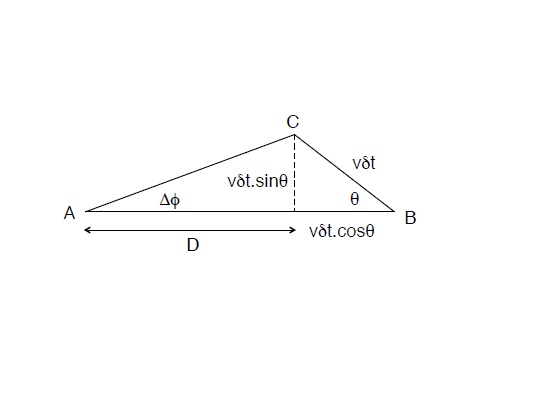
\includegraphics[width=\textwidth]{slum.jpg}
\end{center}
\caption{Superluminal Motion
\label{fig:slum}}
\end{figure}

A blob of gas at position B emits light, then moves to position C with 
velocity $v$, and emits again.  The observer at position A knows the distance 
D to the blob (which is much greater than the distance the blob moves) and 
can measure $\delta t$ and $\Delta\phi$, a small angle.  The observer will 
measure a velocity in the plane of the sky of 
\begin{equation}\label{eq:beta}
\beta_T=\frac{v_T}{c}=\frac{1}{c}\frac{D\Delta\phi}{\Delta t}
\end{equation}
The angular separation between B and C is 
\begin{equation}\label{eq:phi}
\Delta\phi=\frac{v\delta t\sin\theta}{D}
\end{equation}
If the first emission from the blob is at $t=0$, then this light will 
reach the observer at $t_1=\frac{D+v\delta t\cos\theta}{c}$.  The second 
emission will occur at $t=\delta t$ and be observed at 
$t_2=\delta t+\frac{D}{c}$.  The observed time difference will then be
\begin{equation}\label{eq:t}
\Delta t=t_2-t_1=\delta t+\frac{D}{c}-\frac{D+v\delta t\cos\theta}{c}
=\delta t(1-\beta\cos\theta)
\end{equation}
Plugging Equation \ref{eq:phi} and \ref{eq:t} into \ref{eq:beta} gives 
\begin{equation}
\beta_T=\frac{\beta\sin\theta}{1-\beta\cos\theta}
\end{equation}
which can be greater than $1$.

